%!TEX root = ../../diss.tex
\chapter[Foundations]{Foundations}\label{chap:rw:passwords}
%lingo: adversaries statt attackers

% general broad description of where passwords play a role and what authentication is.
Passwords are but one puzzle piece in the realm of cyber security. They are part of the access control paradigm, which is commonly divided into three steps: identification, authentication, and authorization \cite{Riley2006IdentityAuthenticationDistinct}. Identifying a user is usually done with a prompt for a user name, so the system tries to answer the question ``who are you?''. Authentication is about proving that a user -- or more broadly an entity -- is who they claim to be, i.e. authentication is about verification of an identified entity. In other words, the system asks ``How can you prove that you are who you claim to be?''. This verification process can be based on three central elements, namely something that you know (any kind of secret), something that you are (any kind of property), or something that you have (any kind of secret token). One could argue that the second category could be extended by ``something that you do?'', e.g. provide your individual signature. However, authentication does not necessarily \textit{require} identification as a first step. It is well possible to authenticate entities even if they are anonymous. One everyday example are passwords for WiFi networks: Most of the time, the access point does not require a user name; the password, or pre-shared key, in a WPA protocol is enough to join the network. 
Last, authorization is the decision over which resources an authenticated entity is allowed to use, or an answer to ``can the user access this?''.


For this thesis, \textbf{authentication} remains the center of attention. In this chapter, we take a look at various forms of authentication and establish an argument as to why ``something that you know'' is still the most prevalent and significant authentication paradigm to date. 

\section{A Brief History of Passwords}
% first passwords were those on CTSS
The idea of protecting resources with ``something that you know'' is hundreds of years old. Think about the magic words ``open, Sesame!'' that Ali Baba spoke to enter a den used as treasury by forty thieves\footnote{Ali Baba is a fictional character in a story from ``Thousand and One Nights'' as recorded by Antoine Galland in the early 18th century. \url{http://www.pitt.edu/~dash/alibaba.html} \la{16.12.2017}}. The story already illustrates password misuse, because Ali Baba was not the rightful owner of the den and he impersonated the thieves. Nonetheless, this authentication paradigm was brought to the digital world in the early 1960s by the Massachusetts Institute of Technology (MIT) \footnote{\url{https://www.wired.com/2012/01/computer-password/}, \access{16.12.2017}}. Researchers had built a mainframe computer that was programmable by multiple users. At the time, one of the most valuable resources beside the physical device was the \textit{time} granted to use the machine. Thus, the Compatible Time Sharing System (CTSS) was conceived to give every user a certain quota of hours to operate the computer. The quota was enforced by creating user accounts that were password protected. The interaction very much resembles what we still use today: after typing the user name, the password is requested and hidden from the screen during entry.



% First flaws were evident, when the first attack happened
Shortly afterwards, the flaws of the system started to become evident when Alan Scherr became the first ``hacker''\footnote{\url{https://www.slideshare.net/CAinc/history-of-the-password/7-In_1962_a_software_bug} \la{16.12.2017}}. He desired more usage time, so he needed to impersonate other users of the computer and use their quota. The list of passwords on the system was not well protected, which allowed him to access the credentials and carry out what was probably the first password exploit in computer history. Scherr benefited from the fact that passwords were kept in plain text and could be accessed with a special punch card. Interestingly the attack was not detected immediately. Morris and Thompson mention strange behavior in their 1979 paper and blame the issue on a ``software design error'' \cite{Morris1979PasswordSecurity}, while in fact it was Scherr who was responsible for it \ar. 
% now we have cryptop
With the rise of the UNIX operating system in the 1970s, encrypted passwords became standard. The most important algorithm was the Data encryption standard (DES) which was developed by IBM and propagated by the US National Bureau of Standards (today called the National Institute of Standards and Technology, NIST) \cite{Bishop1995ProactivePasswordChecking} \ar. This algorithm was widely used until the late 1990s when computing power was sufficient to efficiently carry out attacks, which rendered DES infeasible. Luckily, the Advanced Encryption Standard had already been proposed and replaced DES. \ar
%TODO maybe add a remark about ``important'' passwords (super user / root) passwords

%TODO more cryptography ?

%%%%%% TABLE BENEFITS AND DRAWBACKS OF PASSWORDS
% Table generated by Excel2LaTeX from sheet 'Sheet1'
\begin{table}[H]
  \centering
  \caption{\label{table:rw:benefits_drawbacks_pws}Benefits and Drawbacks for different stakeholders in a password-based authentication. SPs = service providers.}
  \resizebox{\linewidth}{!}{
    \begin{tabular}{llr}
	\cmidrule{1-3}    Stakes & \textbf{Benefits} & \multicolumn{1}{l}{\textbf{Drawbacks}} \\
	\cmidrule{1-3}    \rowcolor[rgb]{ .949,  .949,  .949} \textbf{SPs} & Low costs & \multicolumn{1}{l}{Large number of attack vectors} \\
	\rowcolor[rgb]{ .949,  .949,  .949}       & Easy to implement & \multicolumn{1}{l}{Anomaly detection costly} \\
	\rowcolor[rgb]{ .949,  .949,  .949}       & Replaceable when compromised & \multicolumn{1}{l}{Attacks are simple to carry out} \\
	\rowcolor[rgb]{ .949,  .949,  .949}       & Revocable by administrator & \multicolumn{1}{l}{Attack automation simple} \\
	\rowcolor[rgb]{ .949,  .949,  .949}       & Enforceable policies & \multicolumn{1}{l}{Attacks can have severe consequences} \\
	\rowcolor[rgb]{ .886,  .937,  .855} \textbf{Users} & Fast entry on desktops & \multicolumn{1}{l}{Memory overload from too many passwords} \\
	\rowcolor[rgb]{ .886,  .937,  .855}       & Most users already familiarized & \multicolumn{1}{l}{Suboptimal coping strategies} \\
	\rowcolor[rgb]{ .886,  .937,  .855}       & Easy to learn & \multicolumn{1}{l}{Stronger passwords difficult to memorize} \\
	\rowcolor[rgb]{ .886,  .937,  .855}       & Sharable with others & \multicolumn{1}{l}{Entry on mobile devices difficult} \\
	\rowcolor[rgb]{ .886,  .937,  .855}       & High degree of control / freedom & \multicolumn{1}{l}{Mastery difficult} \\
	\rowcolor[rgb]{ .886,  .937,  .855}       &       & \multicolumn{1}{l}{Disliked by many users / perceived as burden} \\
	\rowcolor[rgb]{ .851,  .882,  .949} \textbf{Misc} & Independent of identification & \multicolumn{1}{l}{Weak passwords are a risk for users and SPs } \\
	\rowcolor[rgb]{ .851,  .882,  .949}       & Adjustable security level &  \\
	\end{tabular}%
	}%end resizebox
\end{table}%
%%%%%% 

% we were happy with what we had on the system side, so we used it a lot especially on the web.
Around 50 years after CTSS, one of its creators, Fernando Corbató, said in an interview with the Wall Street Journal that password-based authentication has ``become kind of a nightmare with the World Wide Web''\footnote{\label{foot:corbato_regrets}\url{http://on.wsj.com/1sVQOIv}, \access{18.12.2017}}. The surge of the Web has lead to many services requiring authentication. Alphanumeric passwords were the go-to solution because the system is easy to implement and has almost no set-up costs other than a database. This has led to passwords becoming the de-facto standard for authenticating users on the Web.

% passwords do have drawbacks, which is why people have started to look into ways to replace them.
However, passwords do have shortcomings for all the stakeholders involved in the authentication, e.g. Consequently, there have been many attempts to replace passwords to either minimize security risks, make things easier for the users, or -- ideally -- both at the same time. To this point, though, no alternative authentication mechanism has been able to replace alphanumeric passwords on the web, which we investigate in detail in Section \ref{sec:rw:authentication_without_pws}. Put short, the benefits provided by passwords outweigh the drawbacks most of the time. Table \ref{table:rw:benefits_drawbacks_pws} has a high-level overview of the benefits and drawbacks.


%more history in the introduction of \cite{Bishop1995ProactivePasswordChecking}, and of course as early as 1979 \cite{Morris1979PasswordSecurity}


\section{Attacks on Passwords}\label{sec:rw:attack_vectors}
As mentioned above, computer passwords were attacked shortly after they were called into action. Attacks have since become more sophisticated. In the first attack on passwords, Scherr benefited from very weak protection and was able to simply print the passwords and hack into the system. Nowadays, an attacker, or ``the bad guy'' as Morris and Thompson used to call them \cite{Morris1979PasswordSecurity}, has a number of ways to obtain a user's password(s).


%% Attack Overview Infographic
\begin{figure}[h!]
	\centering
	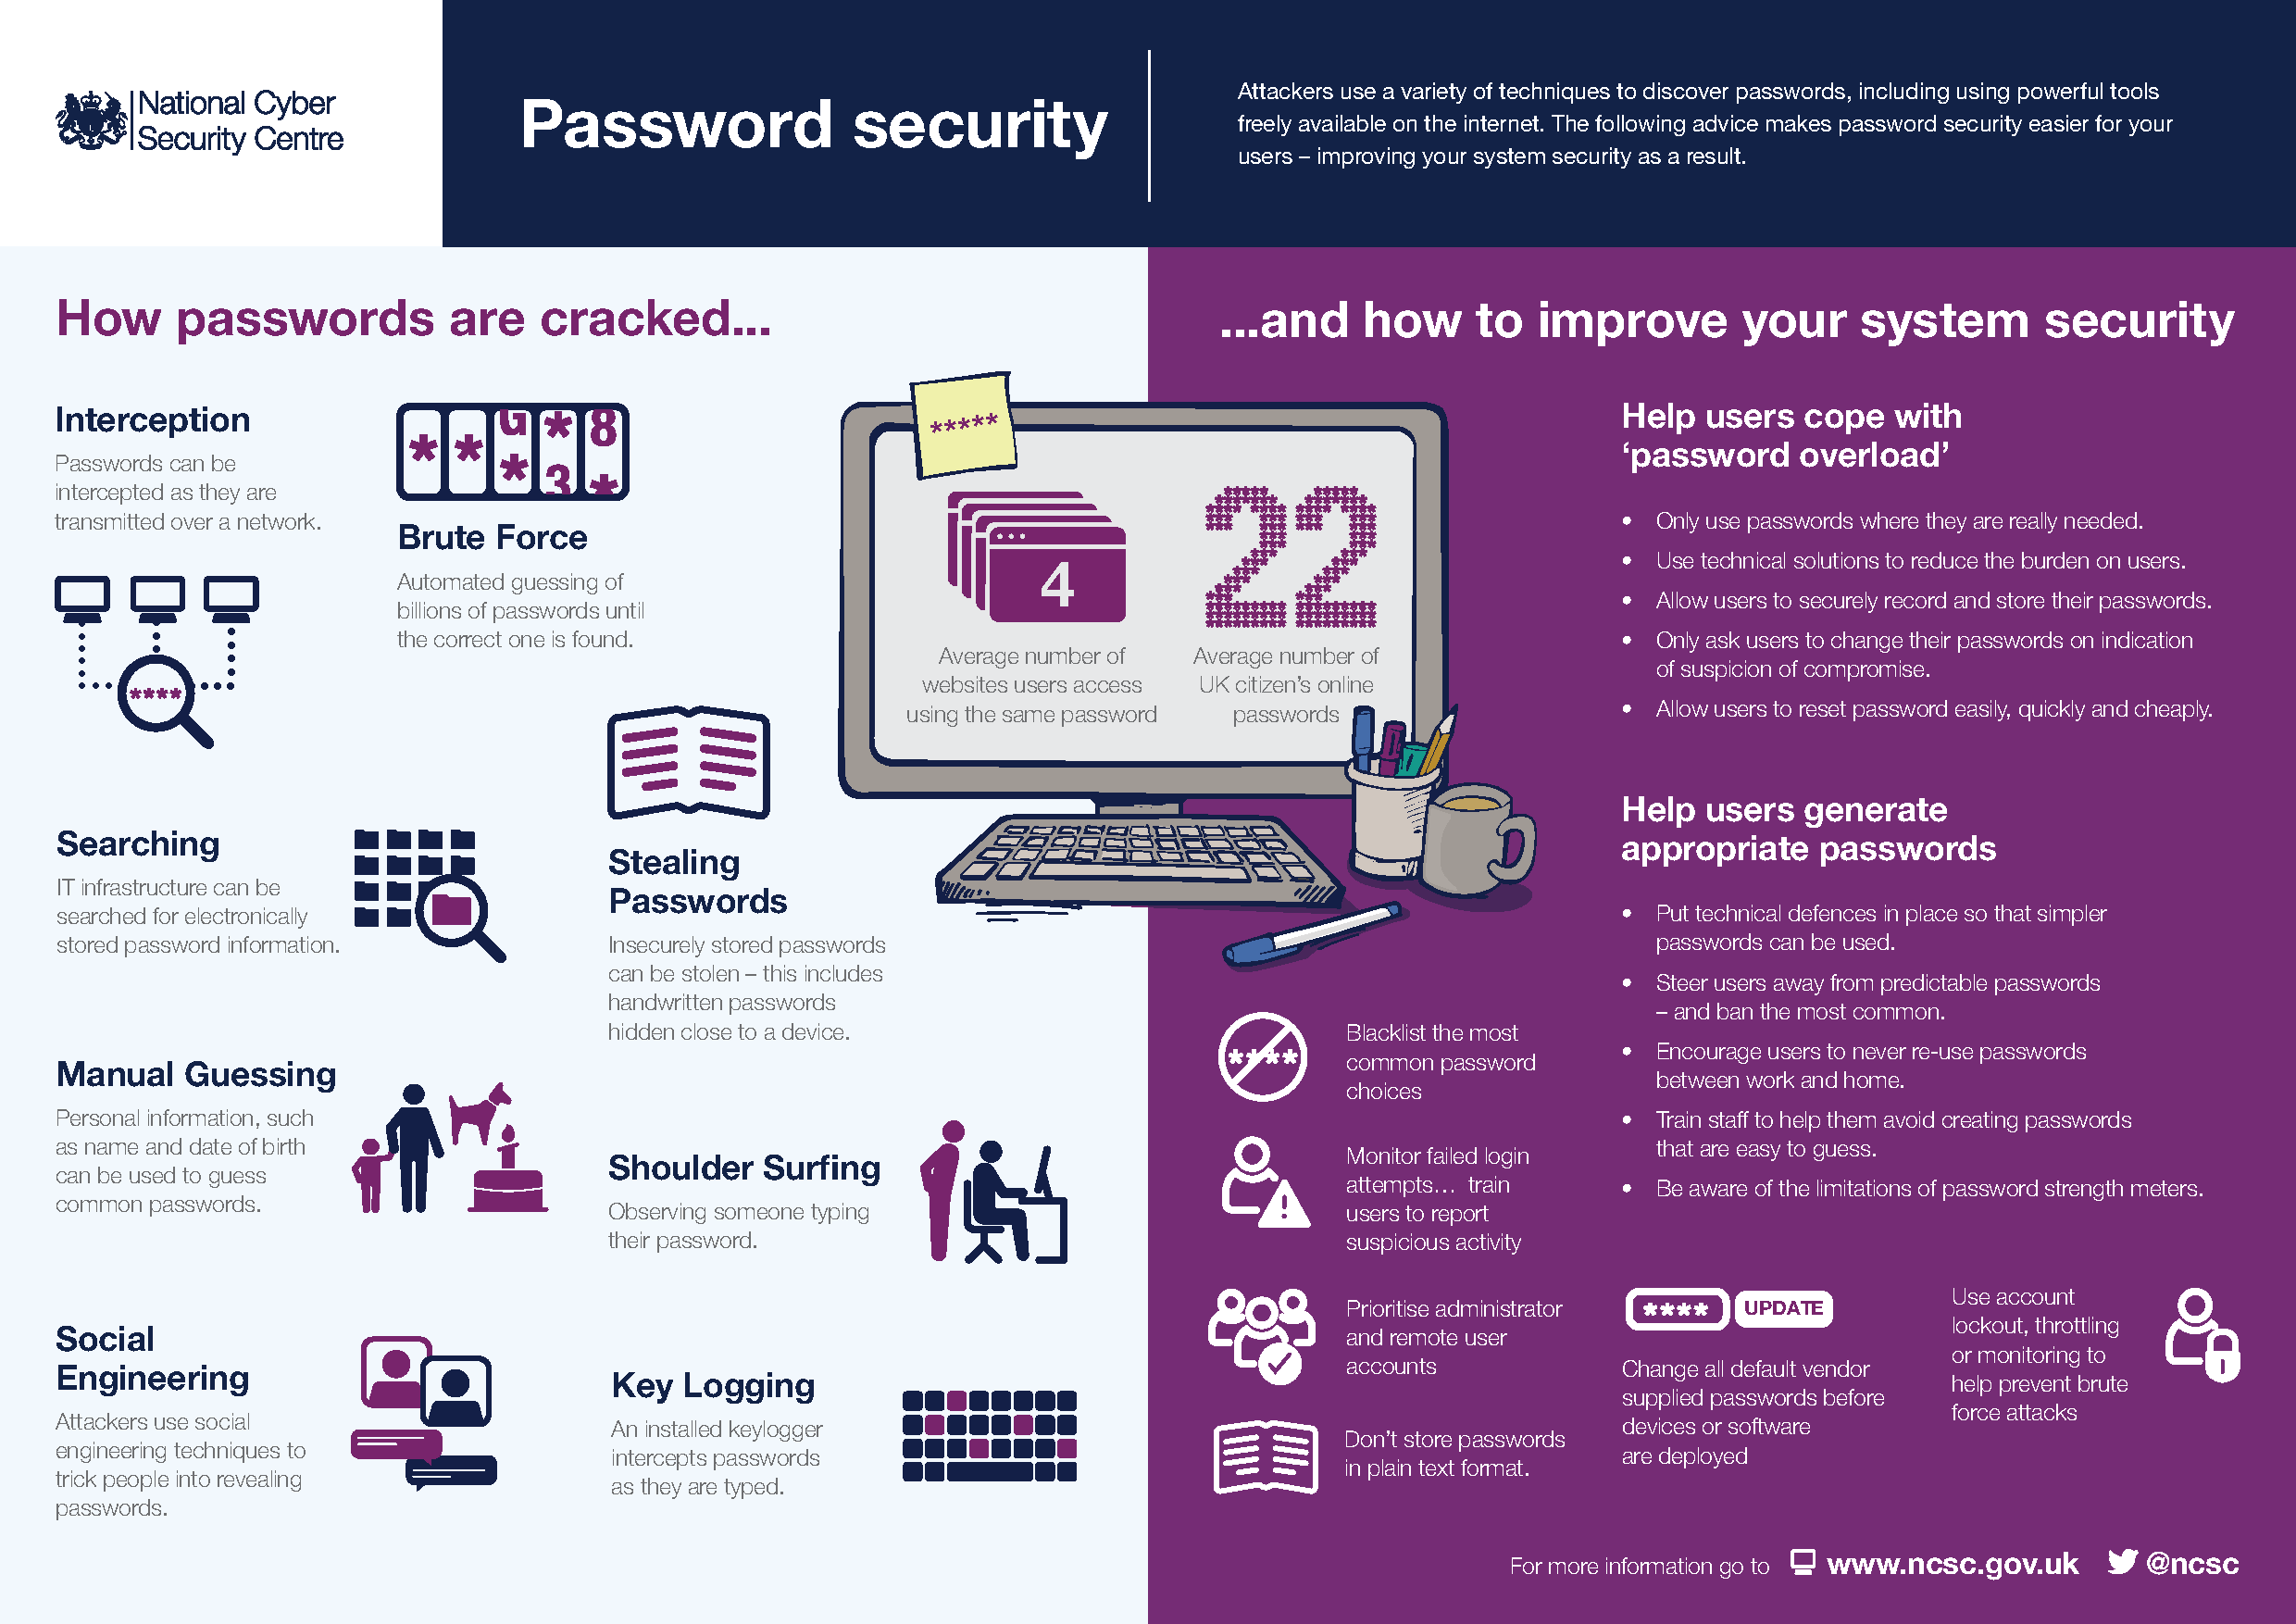
\includegraphics[width=\linewidth]{rw/NCSC-password-security-infographic}
	\caption{
		\label{fig:rw:attacks_infographic}
		Overview of attacks and high-level mitigations. Image courtesy of the National Cyber Security Centre, UK \protect\url{https://www.ncsc.gov.uk/guidance/password-collection} \protect\la{21.12.2017}
	}
\end{figure}



% A short overview of the security threats:
\paragraph{Online Guessing} An adversary tries to impersonate the user by trying different combinations of user names and passwords, which are sent to the authenticating service directly. If successful, the attacker can log in without the user noticing and steal personal information, act on their behalf, and try to use the credentials on other services as well. This attack, which is commonly known as an ``online attack'', is in many cases thwarted by throttling the number of unsuccessful login attempts per account. The service provider can lock down a user account entirely after a given number of failed login attempts. Afterwards, the user either has to manually reset their password, or they need to wait a certain time until the account is unlocked and new login attempts can be made. In the latter scenario, a strategy to hamper attacks is to implement a \textit{backoff} algorithm\footurl{https://devcentral.f5.com/articles/implementing-the-exponential-backoff-algorithm-to-thwart-dictionary-attacks}{20.12.2017} as is done in computer networks, e.g. in the Ethernet protocol \cite[p. 285]{Tanenbaum2011ComputerNetworks}. The idea behind this scheme is to (exponentially) increase the time a user (or attacker) has to wait until they can log in again after the account is locked down. Brostoff and Sasse suggest to allow ten attempts until the account is locked \cite{Brostoff2003TenStrikes}. This should give users enough trials to recover go through their list of passwords which is usually shorter than ten \cite{Florencio2007LargeScaleStudyPasswordHabits}. Perhaps, online guessing is only feasible for determined attackers who target specific victims, but this type of attack is not entirely uncommon \cite{Florencio2013WhereDoAllTheAttacksGo, Florencio2014PasswordPortfoliosFiniteUser, Herley2015Counterfactuals, Wang2016TargetedGuessingUnderestimated}. It is sometimes argued that such an attacker might automate up to 1 Million guesses until the attack becomes infeasible because it simply takes too long \cite{Bonneau2015ImperfectAuthentication, Florencio2014AdministratorsGuide}. However, if the login attempts are not throttled, this can lead to massive attacks, like the largest attack on WordPress to date in December 2017\footurl{https://www.wordfence.com/blog/2017/12/aggressive-brute-force-wordpress-attack/}{21.12.2017}. Florêncio \etal argue that users are well advised to pick passwords that can at least withstand this type of attack, because it becomes too difficult to fend off offline guessing anyhow \cite{Florencio2014AdministratorsGuide, Florencio2014PasswordPortfoliosFiniteUser, Florencio2016CommACM}. 

\paragraph{Stealing / Offline Guessing} Since online attacks are often impractical due to time consumption, offline attacks have prevailed in recent years\footurl{http://breachlevelindex.com/}{20.12.2017}. 
% scenario and high level description how this attack works
In this scenario an attacker breaks into the server of a service provider, usually by exploiting security holes. If this goes unnoticed, the intruder can often access the entire database containing the user account data. He or she downloads the data to their own machine, which allows them to use cracking tools like John the Ripper\footurl{http://www.openwall.com/john/}{20.12.2017}, or hashcat\footurl{https://hashcat.net/hashcat/}{20.12.2017}. These sophisticated tools use dictionaries, mangling rules and brute force to calculate password hashes which are then compared to the entry in the database. If the hashes match, the password was cracked and its plain text version is written to a file. 
% how a service provide would need to protect the data.
Optimally, the passwords in the database are salted and hashed with a slow hash function like bcrypt \cite{Provos1999bcrypt}, which drastically reduces an attacker's chances to crack the password. At the other side of the spectrum, the passwords could be stored in plain text, which would not require any cracking automation at all. Unfortunately, some of the most famous data leaks revealed that data was stored in plain text. 
% real-world examples of data breaches. first: plain text leak at RockYou
The RockYou breach in 2009 contained 32 Million user accounts for its gaming website with plain-text passwords \cite{Bonneau2012ScienceOfGuessing, Weir2010MetricsPolicies}. At the time, RockYou developed games for MySpace and Facebook and the database also contained credentials for these sites\footurl{https://techcrunch.com/2009/12/14/rockyou-hack-security-myspace-facebook-passwords/}{20.12.2017}, which made the leak even more severe. Strong passwords would not have helped at all to avoid losing personal data. Perhaps RockYou's loose policy (5 characters) helped in safeguarding other accounts where more complex policies were in place, because users were not able to reuse their RockYou password there. 
% hashed leaks
In other instances of stolen password databases, the passwords were indeed hashed, e.g. the infamous LinkedIn breaches\footurl{http://fortune.com/2016/05/18/linkedin-data-breach-email-password/}{20.12.2017} -- again with millions of rows of user data \cite{Huh2017TooBusy}. 
% User perspective
Users are challenged to find a password that withstands this kind of attack. The large issue is that attackers are basically only limited by the time they want to spend calculating password hashes. On modern machines with a single GPU, thousands of hashes can be calculated per second even for slow algorithms\footurl{https://gist.github.com/epixoip/9d9b943fd580ff6bfa80e48a0e77520d}{20.12.2017}. Perhaps, this is why Florêncio \etal argue that it is futile to encourage users to pick a password that would withstand such an attack \cite{Florencio2014AdministratorsGuide, Florencio2016CommACM}. 

%% PHISHING WEBSITE SCREENSHOT
\begin{figure}[h!]
	\centering
	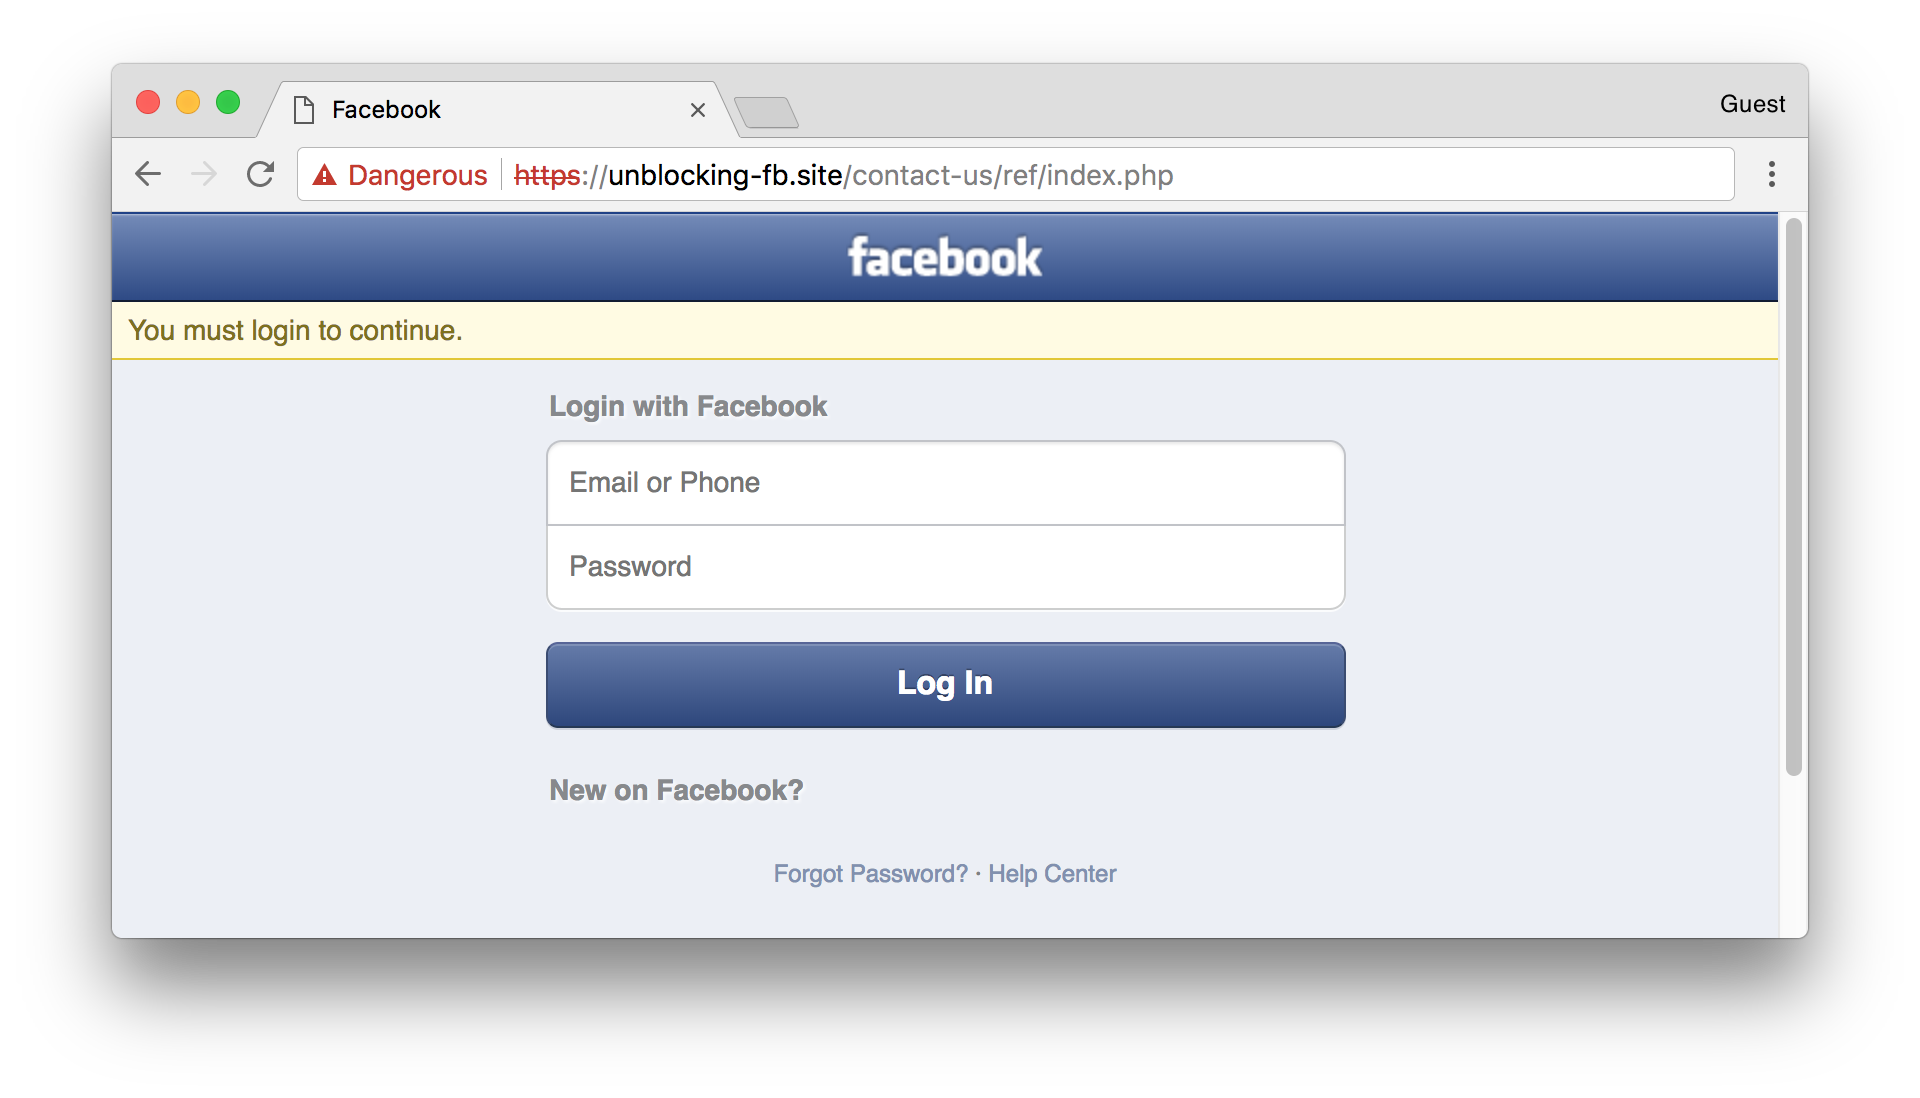
\includegraphics[width=0.7\linewidth]{rw/facebook-phishing-site}
	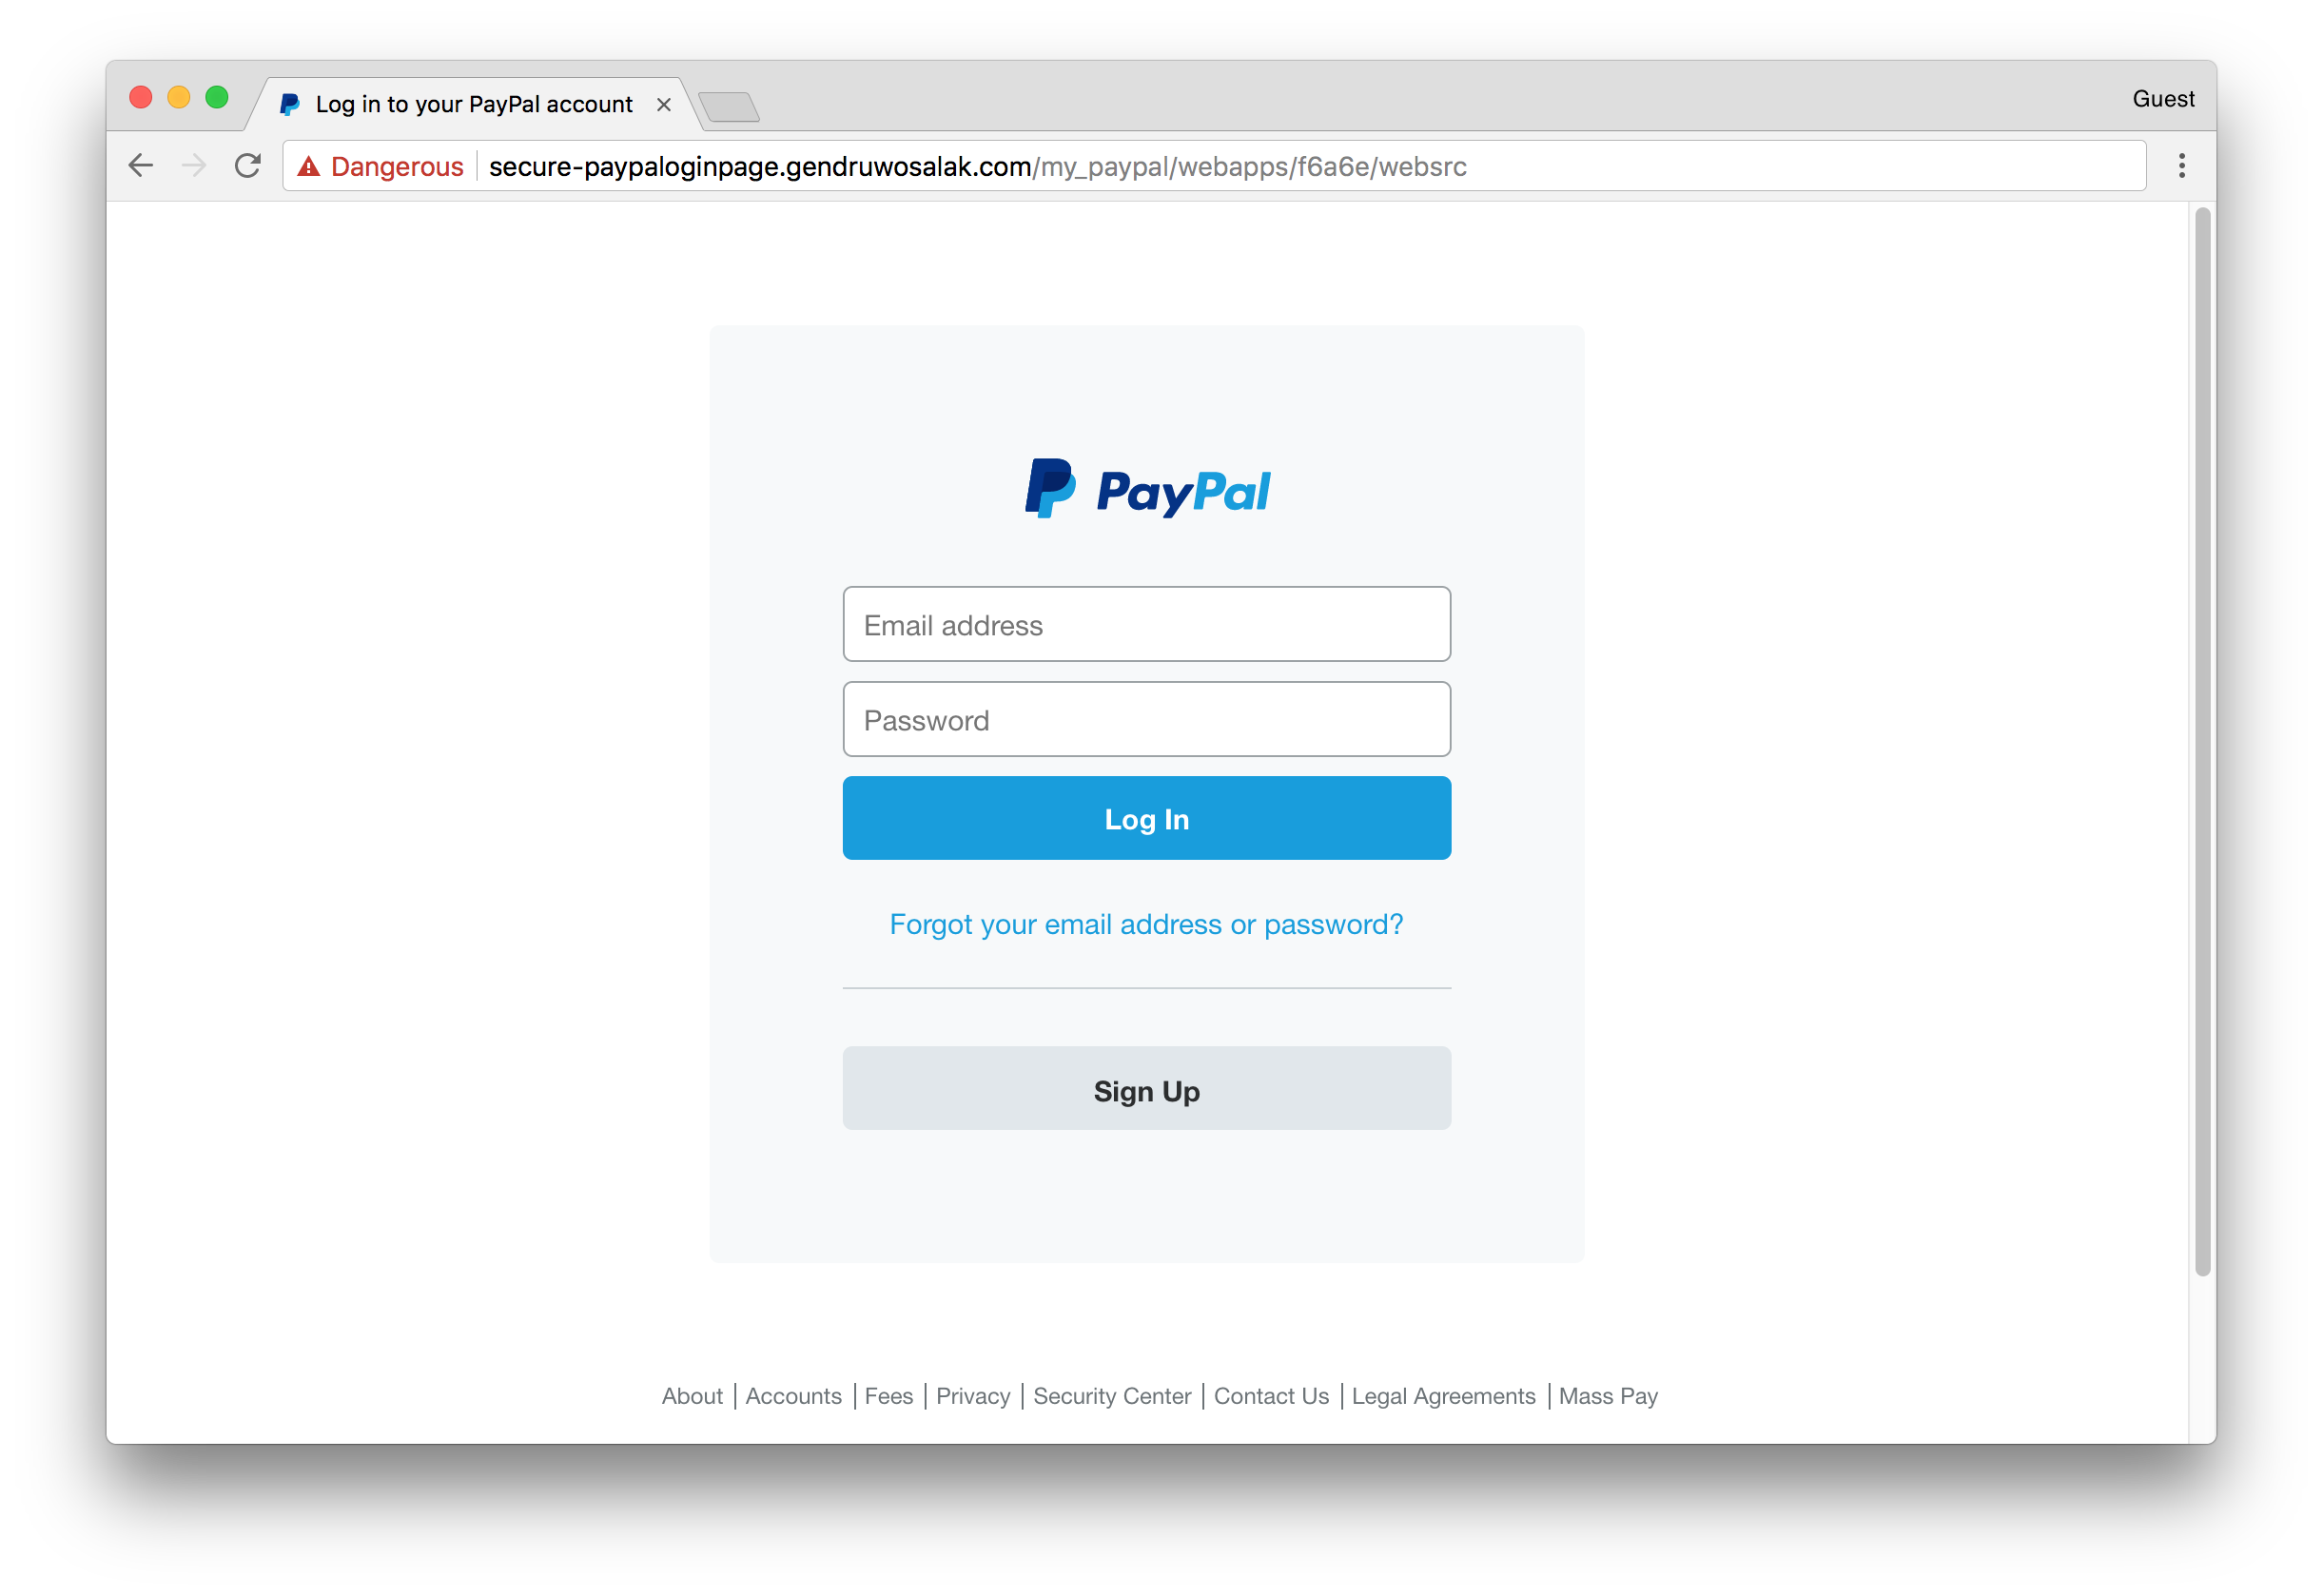
\includegraphics[width=0.7\linewidth]{rw/paypal-phishing-site}
	\caption{\label{fig:rw:phishingsite} Actual phishing websites targeting the facebook and paypal (online and accessible on 21.12.2017). The URLs contain ``fb'' (short for facebook) and keywords like ``secure'' ``paypal'' which contribute to falsely trusting the authenticity of the sites.\todo{propably split into two figures}}
\end{figure}

\paragraph{Phishing / Social Engineering} Social engineering has become one of the biggest threats for a user's passwords with a growing number of incidents and fierce financial damage \cite{BKA2016Bundeslagebild}. Former criminal hacker Kevin D. Mitnick, who calls himself a social engineer, defines the term like this:
\begin{quotation}
	``Social Engineering uses influence and persuasion to deceive people
	by convincing them that the social engineer is someone he is not,
	or by manipulation. As a result, the social engineer is able to take
	advantage of people to obtain information with or without the use of
	technology.'' \cite[Frontmatter]{Mitnick2003ArtOfDeception}
\end{quotation}
Put simply, an attacker fools a victim into revealing certain kinds of information, including passwords. The most common social engineering attack on passwords is phishing, which typically involves two components: a fraudulent website that mimics another service and an email that lures the user onto this website \cite{Dhamija2006WhyPhishingWorks,Sheng2010WhoFallsForAPhish}. The email usually utilizes persuasive techniques like scaring  (``we noticed someone logged into your bank account and you need to reset your password'') time pressure (``you need to act \textit{now} to avoid further damage''). If the website looks just like the original (like the webpage in Figure \ref{fig:rw:phishingsite}), users might fall for it and enter their password to log in. In that case, it does not matter whether it is a strong, complex password or simply 12345 -- the attacker knows the username/password combination from that point on. If this tuple is used on other services, the attacker immediately gains access to them as well. 
% user perspective and mitigations
It is very challenging for users to validate the authenticity of a given webpage \cite{Dhamija2006WhyPhishingWorks, Fogg2001WhatMakesSitesCredible}. Usually, the URL is the best indicator, Dhamjia \etal among others argue that it is unrealistic to keep an eye on the URL at all times. Since the URL and padlock-icons are often ineffective, much research has been dedicated to help users in this validation and prevent phishing attacks. For example, Lin \etal found that domain highlighting in the URL bar only has a small effect on the effectiveness of phishing attacks, even after their participants were explicitly instructed to take not of the URL \cite{Lin2011DomainHighlighting}. Wu \etal showed that browser toolbars do not really help users, either \cite{Wu2006SecurityToolbars}. Dhamija \etal proposed a \textit{trusted path} between the user and the legitimate service \cite{Dhamija2005DynamicSecuritySkins}. In this system, users are supposed to verify the authenticity of a given website by comparing visual patterns in a trusted window and on the website. Together with Max-Emanual Maurer and Alexander De Luca, I created a browser extension to visualize the usage of different types of SSL certificates across websites through the entire browser skin \cite{Maurer2011ShiningChrome}. We deployed it publicly and launched a feedback survey, which indicated that changing the browser skins is obtrusive enough to raise awareness and makes users more confident while browsing the Web. Until the recent change of platform APIs\footurl{https://blog.mozilla.org/addons/2017/11/20/extensions-in-firefox-58/}{21.12.2017} and resulting incompatibility problems, the extension named ``SSLPersonas'' had seen 47000 downloads, which is an indicator of both the necessity and the success of our solution. 

However, optimally the browser would detect phishing websites and prevent that users visit them in the first place. Current versions of the major browsers try to do this and urge the user to leave the site, as is shown in Figure \ref{fig:rw:browser_warning}. This gives attackers only a short time-frame until the webpage has been classified as phishing, which takes around 4-8 hours according to a recent Webroot report \cite{Webroot2017PhishingReport}. Older sources report a bit longer lifespans between 20 hours\footurl{https://www.lightbluetouchpaper.org/2007/05/16/how-quickly-are-phishing-websites-taken-down/}{21.12.2017} and 54 hours\footurl{https://news.netcraft.com/archives/2004/08/14/life_span_of_a_phishing_site_averages_54_hours.html}{21.12.2017}. 

%%%%
%%%% Browser Warning deceptive website.
\begin{figure}
	\centering
	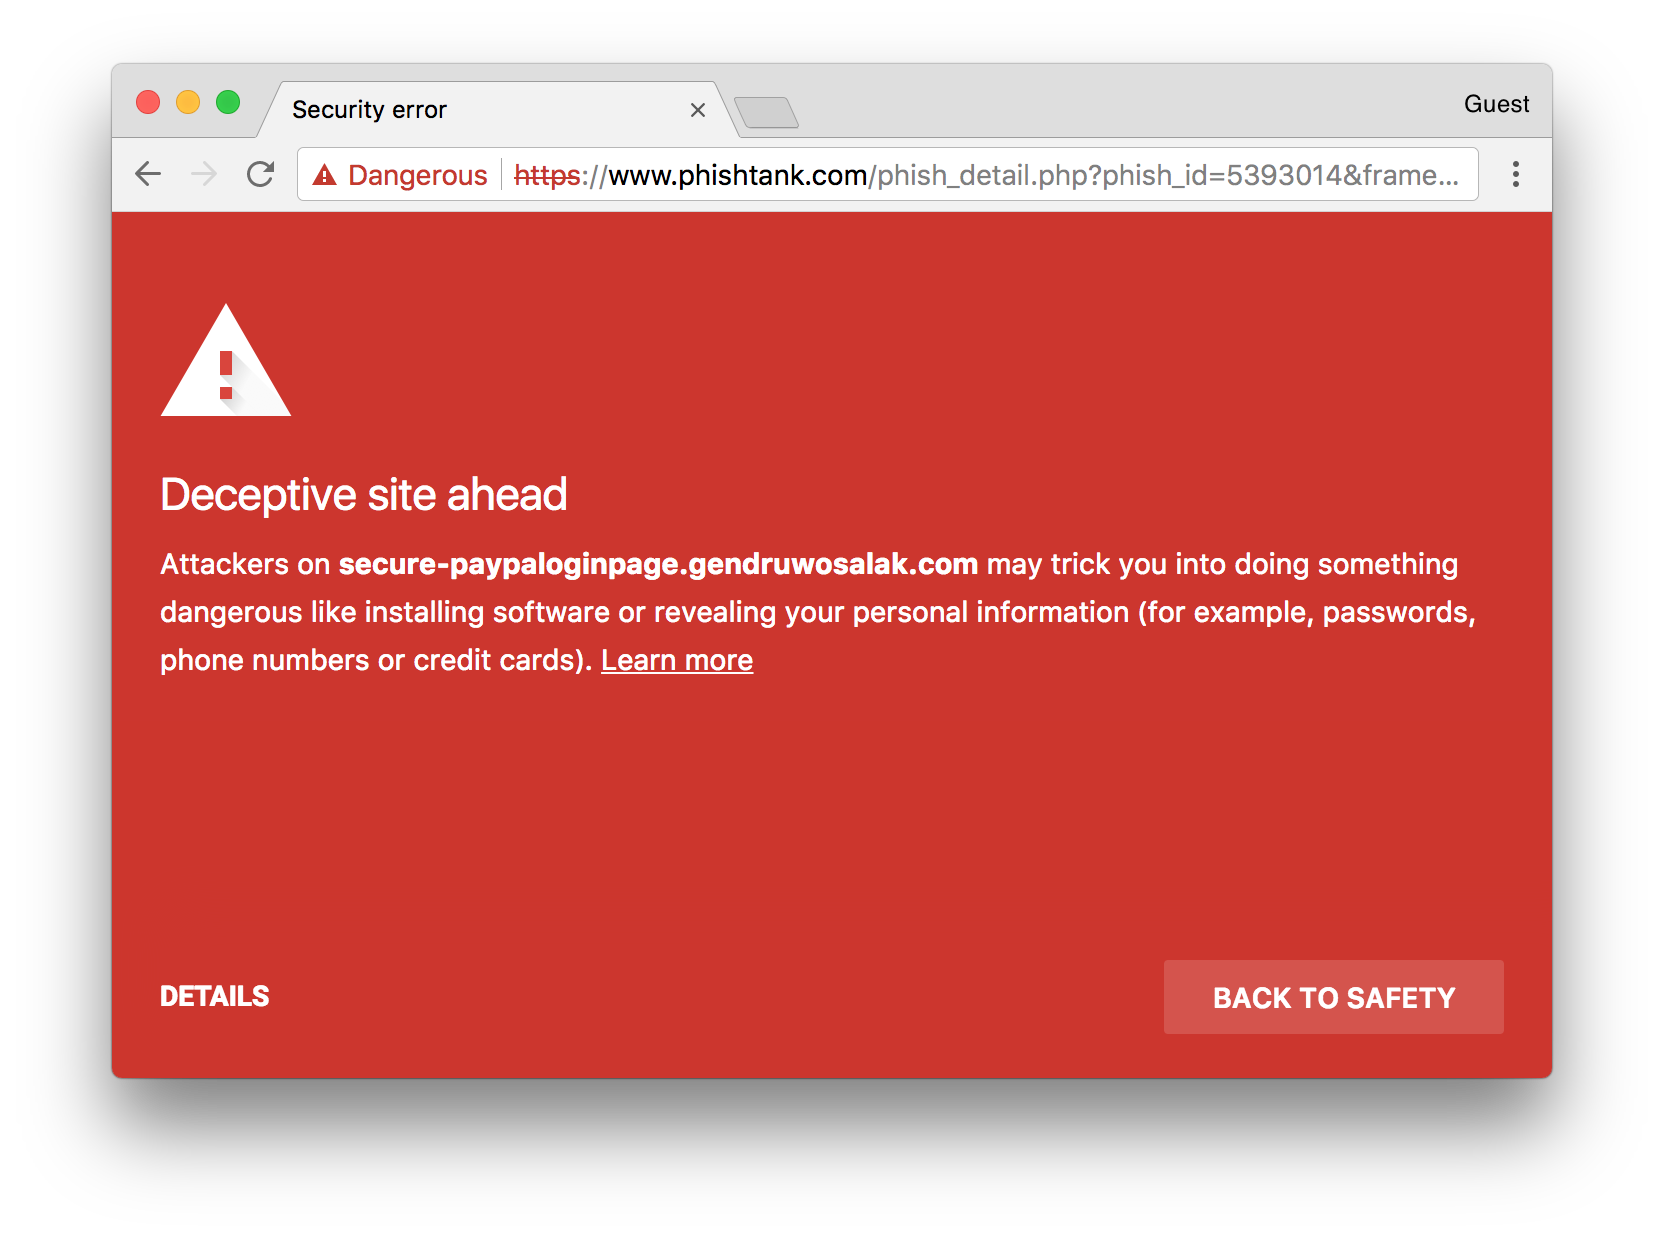
\includegraphics[width=0.8\linewidth]{rw/browser-warning-deceptive-site}
	\caption{\label{fig:rw:browser_warning}Chrome v63's warning on a phishing website. The user is urged to leave the site but still has the chance to visit it by clicking on ``Details''.}
\end{figure}

\paragraph{Malware and Eavesdropping} Secretly stealing plain-text passwords is also possible by infiltrating the user's system with \textit{malware}, which is a term for \textit{mal}icious soft\textit{ware} \cite{Bayer2009CurrentMalware}. One of most common attacks is to install a keylogger that sends all keystrokes to the attacker. For the most part, this either happens as a ``drive-by-download'' when the user visits an infected website or by opening a malicious email attachment \cite{BKA2016Bundeslagebild}. Wash identified that users are aware of this kind of threat, but their mental model of malware is subpar \cite{Wash2010FolkModels}. Hence, the countermeasures taken by the users are often insufficient. As with the phishing scenario, a strong password is incapable of preventing a malware attack. Ideally, users use an anti-virus solution, keep their software updated at all times and refrain from opening suspicious email attachments. 

Moreover, user credentials can be intercepted in transit, e.g. after the user submits them through a web form. These so called man-in-the-middle attacks are tough to carry out, but strong passwords do not prevent them either. One of the typical solutions to minimize the risk is encrypting the traffic with a secure protocol like SSL/TLS \cite[p. 853ff.]{Tanenbaum2011ComputerNetworks}, which is based on a public/private key infrastructure. This makes it harder for an adversary to act as the man in the middle, because they usually do not possess the necessary private key of either party. Attackers must tamper with the certificates which usually causes browsers show a warning \cite{Maurer2011ShiningChrome}. Users, however, do not necessarily understand such warnings, because their understanding of the technical details is low \cite{Herley2009SoLongThanksExternalities, Whitten1999WhyJohnnyCantEncrypt}. Consequently, the HCI community has invested much effort to convey the essential messages in a clear and actionable way \cite{Felt2015ImprovingSSLWarnings, Felt2014ChromeSSL,  Maurer2011ShiningChrome, Sotirakopoulos2011ReplicationSSLWarnings, Sunshine2009CryingWolf}.

%Keyloggers, eavesdropped communication (e.g. via Man in the Middle Attacks)

\paragraph{Observation} 

Shoulder surfing, passwords on post-its at the office. that's why passwords are masked in the browser (with an asterisk per character), but the benefit has recently been questioned \cite{Sasse2016DebunkingMyths}. 

\paragraph{Other attacks} 
Apart from the attacks described above, there are other approaches that should not go unmentioned. First, people in one's own social circle, e.g. friends and family, have much personal information and often physical access to devices. Although the intent is often not purely malicious, it can be easy for these people to have an informed guess of a user's credentials. Flechais \etal use the term ``spouse attack'' to describe this kind of threat \cite{Flechais2013SaudiArabiaTrust}. A strong, complex password that is only memorable to the legitimate user might help in that scenario. Weirich and Sasse, however, argue that such a strategy could make the user appear ``paranoid'' \cite{Weirich2001PrettyGoodPersuasion} and Flechais \etal see it as an important sign of trust \cite{Flechais2005DivideConquerTrust, Flechais2013SaudiArabiaTrust}. 
 

stealing (on GitHub, npm problematic) -- mitigations: 2FA // or  locally on post it notes: mitigation secure place. 

%%%% 
%%%% TABLE: Attacks and Countermeasures
% Table generated by Excel2LaTeX from sheet 'attacks-mitigations'
\begin{table}[htbp]
  \centering
  \caption{\label{table:rw:attacks_countermeasures}Threats on passwords and potential countermeasures for users and service providers (SP). Other stakeholders are left out of this analysis.}
    \begin{tabular}{rll}
    \multicolumn{1}{l}{\textbf{Threat}} & \textbf{Countermeasures} & \textbf{Responsible} \\
    \hline
    \multicolumn{1}{l}{\textbf{Online Attack}} & Throttling & SP \\
          & Anomaly detection & SP \\
          & Set-up Multi-factor authentication & SP \\
          & Moderately complex password & User \\
          & Enable Multi-factor authentication & User \\
    \multicolumn{1}{l}{\textbf{Offline attack}} 
        	& Slow hash algorithm & SP \\
			& Secure database design & SP \\
			& Security audits, fix vulnerabilities & SP \\
		    & Complex, strong password & User \\

    \multicolumn{1}{l}{\textbf{Phishing}} & Education and Warnings & SP \\
    & Unique passwords & User \\
          & Check security indicators & User \\
          & Utilize spam filter & User \\
          & Vigilance regarding emails & User \\
    \multicolumn{1}{l}{\textbf{Malware}} & Anti-Virus software & User \\
          & Caution on the web & User \\
    \multicolumn{1}{l}{\textbf{Observation}} & Password masking & SP \\
    	& Awareness of surroundings & User \\
    \end{tabular}%
\end{table}%
%%%%
%%%%

Florêncio \etal proposed a classification for attacks \cite{Florencio2014PasswordPortfoliosFiniteUser}. Class 1-3

what is an attack ``vector''? attack steps from start to success. \ar
Sometimes combinations of attacks (vector)

Who are the attackers in general? ``spouse attacks'', colleagues? \cite{Ur2016PerceptionsPassword}


The main objective of this thesis is combating online and offline attacks, where password coping strategies really make a difference. A panacea for all kinds of threats, each of which has warranted multiple PhD theses, is probably impossible to find. 

\section{What is Password Strength? - Metrics and Statistics}\label{sec:rw:pw_strength_metrics}
Bishop and Klein said in 1995: ``A good password is one that is easily remembered, yet difficult to guess.'' \cite[p. 231]{Bishop1995ProactivePasswordChecking}. The second part of this statement describes password \textit{strength} on a high level. But there are problems if we try to objectively measure the ``difficulty to guess'' a password: is it difficult for an attacker with nearly unlimited resources, or only for an attacker that can only attempt once a day due to lock-out mechanisms? The question is highly context dependent and there is unfortunately no single true answer. 

How to attack passwords
- here the most important paper is \cite{Ur2015MeasuringRealWorldAccuracies} -- mention tools like HashCat/oclHashcat, John The Ripper 

give some real world examples how passwords are attacked online and how they have been attacked offline. 


Lately the community reached widespread consensus that the realistic strength of password can be defined as \textit{the number of attempts that an attacker would need in order to guess it} \cite{Dellamico2015MonteCarlo}

 

Don't forget: Password strength is dynamic! New leaks can render strong passwords very weak. Yang \etal state: ``If a strategy is widely used, then attackers may develop strategy-specific methods which can efficiently guess the passwords.''

Bonneau looked at leaked passwords and tried to attack them in different ways to find patterns in user behavior that could be leveraged in real-world attacks \cite{Bonneau2012ScienceOfGuessing}. Fundamentally, the attacks were based on different dictionaries. He found that the success rates of attacks strongly depend on the dictionary that is used for it. Under the assumption that entropy is a viable strength proxy, he concluded that 10 bits of entropy are probably enough to defend against online attacks, respectively 20 bits for offline attacks. 

\cite{Peisert2013PriciplesAuthentication,Bonneau2012ScienceOfGuessing,Scott1995GDMS,Dellamico2015MonteCarlo,Ur2015MeasuringRealWorldAccuracies,Egelman2015SeBIS,Conklin2004PWAuthenticationSystemPerspective,Schmidt2013Pitfalls,Kelley2012GuessAgain,Mazurek2013Measuring,Weir2010MetricsPolicies}

	\subsection{Entropy vs. Guesswork}
	
	Other definitions: ``The strength of a password should represent the amount of effort an adversary must employ to break the password'' \cite{Carnavalet2014AnalyzingPWStrengthMeters}.
	
	William Burr regrets NIST policy (see footnote \ref{foot:burr_regrets})	
	
	Entropy (Shannon) -- degree of randomness. often too focused on characters and doesn't address human password selection, which is far more predictable 
	(effective vs. theoretical password space)
	
	@@TODO tell the story of all the attacks -- Kelley, Weir, Bonneau, Melicher, Johnson, Ur etc. Password Guessability Service etc. 
	
	Leaked password dictionaries: Most commonly: RockYou (gamer site), MySpace, LinkedIn, Gawker, Yahoo!
	Mark Burnett  \cite{Burnett2005PerfectPasswords} 
	
	Tell the history of how guesswork was modeled. Starts out with \cite{Weir2010MetricsPolicies}, then \cite{Kelley20012GuessAgain} and \cite{Bonneau2012ScienceOfGuessing}. 
	
	NIST entropy was THE measure for password strength until the Weir paper and shortly afterwards. \cite{Komanduri2011OfPasswordsAndPeople} is probably the last CMU paper that uses entropy as strength metric (and is proud of it).
	
	Entropy is relative to / dependent on a given set of passwords. 
	
	\subsection{Beta-guess-rate}
	$\lambda_{\beta}$
	quasi: how likely is it to find the top $\beta$ passwords in a given dataset?
	see bonneau, and also used in \cite{Yang2016MnemonicSentenceBased}
	brostoff and sasse  proposed 10 as a threshold for rate-limiting (before account is locked and password invalidated until reset) \cite{Brostoff2003TenStrikes}
	
	
	
	
	\subsection{Strength Proxies: The zxcvbn Approach}
Daniel Wheeler presented an approach towards password strength estimation by looking at a conservative expected guess attempt number \cite{Wheeler2016zxcvbn}. The idea is to utilize pattern matching against dictionaries and leaked password corpora and then calculate the minimum rank over a series of frequency ranked lists. In other words, the approach is heuristic instead of probabilistic, because the ranking is based on searching through the patterns and ranking them not only based on their likelihoods, but other factors like keyboard sequences. The implementation of the algorithm is called zxcvbn\footnote{The name zxcvbn originates from the bottom row on a QWERTY keyboard. Many users mistakenly consider this approach secure because the resulting password looks fairly random.}. Wheeler showed that in an online attack scenario \cite{Florencio2014AdministratorsGuide} the algorithm estimates the number of guesses accurately within an order of magnitude of 2 -- consistently better than NIST guidelines to date and KeePass strength estimators. That is, utilizing 100,000 tokens stored within a 1.5 Megabyte file zxcvbn conservatively estimates the number of guesses required to crack a password. Beyond the online-attack threshold, the results are mixed, but we can observe that adding more tokens to the dictionary improves accuracy even more. The great benefit of using this method is its speed and size that make it a lightweight tool that is prepared for widespread adoption, to relieve users from ``LUDS'' policies (lowercase, uppercase, digits, symbols). We can conclude that zxcvbn is a reasonable tool when we collect meta statistics about passwords, e.g. in studies where it is ethically questionable to collect plain text passwords \cite{Seitz2016SuggestionsDecoy}. Wheeler also points out that at this point there is no study comparing the effects the different estimators have on user behavior. 

papers that used or mentioned zxcvbn:
\cite{Komanduri2014Telepathwords}
\cite{Wang2016fuzzyPWM}
\cite{Ur2017DataDrivenPWMeter}
\cite{Yang2016MnemonicSentenceBased}
\cite{Gross2016CognitiveDepletion}

Weaknesses \cite{DeCarnedeCarnavalet2015PasswordMeters}: only english dictionary words, fixed dictionary with the constraints of being transfered to the client, so some passphrases are considered strong while they are not really super great, e.g. ``dolce\&gabana''
not true anymore but in the paper: reversed passwords are not recognized (Wheeler updated this). 


\section{What is a ``Bad'' Password?}
This question is flawed, and thus cannot be answered without context. The word ``bad'' is judgmental and depends on whom is asked. A security expert might call a password ``bad'' if it only contains lowercase letters, but a regular mainstream user might call it ``bad'' because they cannot type it quickly or can't remember it well. 

Bishop and Klein said in 1995: ``A good password is one that is easily remembered, yet difficult to guess.'' \cite[p. 231]{Bishop1995ProactivePasswordChecking}

Let's look at 

types of attacks: phishing, online (rainbow), offline, targeted online. \cite{ZhangKennedy2016RevisitingPasswordRules}. 

When does password strength really help? 

This paragraph from Herley and Van Oorschot says it all \cite{Herley2012PersistenceOfPasswords}:
``Fifth, when are off-line attacks a threat? While dependent on implementation, access to salted hashed pass- words requires attacker effort; long gone are the days when password hash files were by default world read- able. A disgruntled ex-sysadmin who steals hashed pass- words is the often-conjectured foe in this attack; yet, if un-trusted individuals have had unfettered unaudited access to the authentication server, a site’s problems go well beyond password strength. Sixth, are there ways to protect against off-line attacks besides password strength? Mandating password changes once hashes leak might be better than strong policies at all times. Only if a leak goes unnoticed (and a password change isn’t forced) does strength potentially help. Of course, reliably detecting leaks or break-ins it- self remains difficult. Finally, how much strength is required to protect against off-line attacks? The bar is clearly much higher than for online attacks (assuming lockout or rate-limiting policies in place), but at what strength are attacks effectively addressed? More strength is always better for security,'' 

discuss online and offline attacks
\cite{Wang2016fuzzyPWM} has an overview/comparison
\cite{Florencio2014AdministratorsGuide} shows models
\cite{Florencio2014PasswordPortfoliosFiniteUser} has math

A problem about only taking ``online'' attacks into account is that they do allow denial of service attacks, for example if there's lockout policy in place that invalidates passwords after 10 failed login attempts, an attacker would only need to take a list of email addresses (readily available on the internet) and run 10 or more guesses per user and lock all of them out at once. 



We shouldn't call it good or bad. A less judgmental terminology is ``strong'' and ``weak'' because this doesn't include opinions. 

A ``strong'' password is one that cannot be guessed easily by a human or a machine, regardless of the level of information they have about the owner of the password. 


The idea behind a PCFG based policy is to reject passwords that are too ``probable''. 

Characteristics of weak passwords \cite{Burnett2005PerfectPasswords}
\begin{enumerate}
	\item Are used by many users
	\item Can be found through an internet search
	\item Are short (6 characters or less)
	\item Have leaked
	\item Are written down where anyone can access them
\end{enumerate}

But there are other, non-technical qualities of passwords that are usually not covered by the weak-strong spectrum. 

When is a password \textbf{``Appropriate''}? This largely depends on the usage context. \cite{Gaw2005ReuseRecycle, Haque2014Hierarchy}
Florencio \etal argue that it is absolutely fine to choose a weak password for ``don't-care'' accounts \cite{Florencio2014}.

Requirements from a user perspective: memorable and easy/fast to type on all devices.

this creates tensions that are discussed in detail in Chapter \ref{chap:rw:user_perspective}.


\section{Authentication without Passwords}\label{sec:rw:authentication_without_pws}
The benefits and drawbacks of using passwords have been studied extensively. Some drawbacks already become apparent when we recall Ali Baba's story: Ali Baba overhears the thieves saying the magic words and can immediately authenticate with them (a big security issue). He also told the ``password'' to his brother, but he fails to recall it (the biggest usability issue).

Table \ref{table:rw:benefits_drawbacks_pws} shows a high-level summary of the benefits and drawbacks that come along with password-based authentication. We can observe that the drawbacks constitute important constraints and it is natural to try to remove such limitations by considering alternatives. This section briefly covers the most notable approaches to authenticate users without alphanumerical passwords.

\begin{table}
	\begin{tabular}{|l|l|l|}
		Benefits | Drawbacks 
	\end{tabular}
	\caption{\label{table:rw:benefits_drawbacks_pws}Benefits and Drawbacks of passwords for different stakeholders}
\end{table}
%benefits: easy to implement, users know how they work, concept is easy to learn, can be shared, can be replaced when they are compromised, can be revoked by the sys admin, quick to enter, work without a user name (WiFi) so it's easy to scale. 
%drawbacks: users have to cope with many passwords, so they use risky strategies \ref{sec:rw:how-users-cope}, it's difficult to manually create a password that is both usable and secure (good enough to protect against offline attacks)




% das passt nicht unbedingt hier rein, ist aber sehr wichtig. 
Bonneau et al. argue \cite{Bonneau2015ImperfectAuthentication} that passwords are an imperfect technology that is difficult to replace. One, industry has found ways to work around the many drawbacks and can compensate breaches to a large part. Second, alternatives to passwords are often privacy invasive. For example, identity providers like Google or Facebook often collect large amounts of personal data on the users. Third, Bonneau et al. point out that empirical evidence from practice often contradicts results produced by academic research. They advocate that researchers rethink their model of users, who often behave too predictably and whose behaviors one should not try to change. Instead, academia could tackle new approaches that would be dangerous to the success of businesses and thus are seldom tried out. 

% noch mehr Zusammenfassung für später:
The authors point out how user models assumed by researchers often do not apply in reality, for instance, their behavior is anything but random: Users pick from a limited set of passwords that is far smaller than random passwords. Just as \cite{Florencio2014PasswordPortfoliosFiniteUser}, the paper strongly discourages focusing on offline attack scenarios and suggests that users should at most try and protect themselves against online attack scenarios. Consequently, the lessons from the past about attempts to improve password strength through changing user behavior are questionable in the authors' eyes. Even more so, because other attacks (phishing, malware, eavesdropping, stealing from servers or identity tokens) are not fended off at all by stronger passwords. Online attacks can drastically be mitigate by rate-limiting and contextual information (e.g. geolocation). Yet, the authors see that not all sites employ these methods, ``probably to avoid denial of service''. Users also often receive too much advice from security experts that is often contradictory and in extreme cases boiled down to ``Pick something you cannot remember and do not write it down''. 

Bonneau et al. answer the question whether we still need passwords with a differentiated ``yes'': \textit{Passwords appear to be a Pareto equilibrium\footnote{\todo{add definition of this here. It's about game theory.}}}. Also the learning curves for password authentication at a new service is virtually non-existent. However, as many researchers in the community, the authors see the feasibility of multi-factor authentication in progressive or continual ways as the most promising future. The challenges for privacy and usability we find in these approaches are mostly ill-defined or not validated. The user experience of such systems may improve while the drawbacks come at a high price that the users may not understand at all. 

	\subsection{Graphical Passwords \& Visual Authentication Methods}
ColorPIN, Ema's work, \cite{Renaud2009VisualSnakeOil} 

	\subsection{Biometrics}
	
	\cite{Jakobsson2014HowToWearYourPW,DeLuca2012TouchMeOnce,Peisert2013PriciplesAuthentication,Rybnicek2014RoadmapContinuousAuth}
	

	fingerprint omnipresent 
	retinal scan
	face recognition (iPhone X)
	
	
	Anecdote to show that it is a bad idea\footnote{\url{https://www.theguardian.com/world/2017/nov/08/qatar-airways-plane-forced-to-land-after-wife-discovers-husbands-affair-midflight}, \access{08.11.2017}}
	
	\subsection{Multimodal and Implicit Authentication}
	
	actually the technical report gives some insights about this \cite{Stockinger2011ImplicitAuthentication}, so that will inspire a bit.
	also look into the USEC folder in the office, the papers and annotations are in there.
	
		it's interesting that the most cited CHI paper of the last 5 years is about implicit authentication \cite{DeLuca2012TouchMeOnce}
	
	Machine learning. Accuracy / Recall / Error rate / True Positve / False Positives etc. -- based on \textbf{probability} and not on \textbf{certainty}. To account for the lack of certainty, in all current state-of-the-art mechanisms passwords serve as fallback authentication. So, while it reduces the number of password entries and so speeds up interactions in many cases, these schemes cannot fully replace passwords. What is worse is that the rare interaction often tempts users to choose a very memorable secret, which in most cases is weaker than a password that is entered on a regular basis. So an attacker that is successfully denied access to a system protected by multimodal authentication will always have the opportunity to authenticate with a password -- the system needs to assume a false negative and offer the fallback authentication scheme. In this scenario, while the primary authentication is more usable and very secure, the entire system's security is lowered by its fallback scheme. This fact is often played down and neglected in the marketing of new multimodal authentication. 
	
	Take away: implicit authentication cannot replace explicit authentication, but it can make an existing scheme more secure. Fallback schemes tend to lower system security. 
	

	
	\subsection{Shared Authentication and Hardware Tokens}
Single Sign-On (SSO). 
Identity Providers, 
SecureID or ``Gnubby'' (see Google)
Two-Factor Authentication / 2-step --> hints to 2-step in ``Some UNIX systems have instituted what is called an "external security code" that must be typed when dialing into the system, but before logging in. If this code is changed periodically, then someone with an old password will likely be prevented from using it.'' \cite{Morris1979PasswordSecurity}

Reference Models:

\cite{Egelman2013ProfilePassword,Sun2010BillionKeys}

\begin{itemize}
\item \textbf{OAuth} Twitter, Google
\item \textbf{OpenID} Google, PayPal
\item \textbf{Facebook Connect} 
\end{itemize}
Problems: 
Successful identity providers such as Facebook take a central role as the ``sole identity provider, which does little for privacy'' \cite{Bonneau2015ImperfectAuthentication}.


\textbf{Privacy} The biggest players for shared authentication are Facebook, Google, and Twitter. However, it is exactly these three companies for which users raise the most privacy concerns. On the one hand, users trust the companies because they know how much data they store and manage, and only few breaches are known. On the other hand, users are doubtful that their credentials will be in safe hands and not shared with third parties (users lack the understanding of how shared authentication works internally and cannot separate privacy and security). 

\textbf{Single Point of Failure} Embracing the opportunities of shared authentication, users integrate it into their password management / coping strategies \ref{sec:rw:how-users-cope}. 

	
\subsubsection{One Time Passwords}

OTP also have the possibility to replace a password that you have to memorize, but there are disadvantages as well. 
illustrate the workflow from Slack.

Authentication Melee paper has some intel on one-time passwords: \cite{Ruoti2015AuthenticationMelee}


\section{Passwords are Here to Stay}
no solution fully replaces them

most approaches that are seen as more usable are often based on probability rather than certainty (TPR / FPR / EER). fallback to passwords probable even for other authentication schemes. everything else is often less usable than passwords. 

maybe discuss this at the end of the thesis: passwords are cool, and we can continue to use them because they are so easy to replace in case of a breach. 

An approach that is currently not undertaken in internal security audits is the following: there are password leaks once a month (see data breach reports). the security team could take the passwords (if they are hashed - crack them first) and invalidate all matching passwords in their own password database. Of course, they need to inform their users. I could sketch a flowchart what this should look like. This would allow reusing passwords more securely without shifting much responsibility to the users. 

``We argue that it is time to admit that passwords will be with us for some time, and moreover, that in many instances they are the best-fit among currently known solutions.'' \cite{Herley2012PersistenceOfPasswords} 

The Herley and Van Oorschot paper really has lots of good quotes and thoughts for this \cite{Herley2012PersistenceOfPasswords}


\cite{Kirlappos2012SecurityEducation,Loutfi2015PasswordsOtherSideOfTheFence,DeAngeli2005PictureThousandWords,Florencio2013WhereDoAllTheAttacksGo,Herley2008ProfitlessEndeavor,Sasse2015,Dittrich2009,Herley2009SoLongThanksExternalities,Vantaggiato2015WeStillNeedPasswords,Florencio2010WhereDoPoliciesComeFrom,Schrittwieser2013,Bonneau2015ImperfectAuthentication,Cyber2014,Florencio2007DoStrongWebPasswords,Sasse2005UsableSecurityPosition,Aebischer2017PicoInTheWild,Forget2007HelpingUsers,Herley2009IfWereSoSmart,Acar2016NotYourDeveloper,Sasse2016,Renaud2009VisualSnakeOil}

